

% \subsection{VAE with MLP Models}

% \subsubsection{VAE-MLP (50 Epochs)}
% During the experimentation phase, three variations of the VAE with MLP were trained and evaluated. The architecture defined in section 3.3.1 was used to train the flattened STFT features.

% Initially, a basic VAE-MLP model was trained for 50 epochs, and its training and validation losses were visualized. Observing the loss plot, both the training and validation loss were decreasing and showed no signs of overfitting or underfitting.

% \begin{figure}[htbp]
%     \centering
%     \begin{minipage}[b]{0.45\linewidth}
%         \centering
%         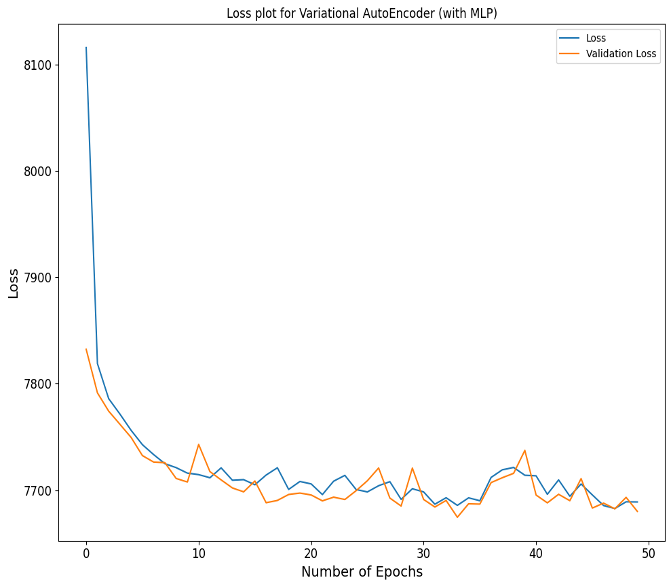
\includegraphics[width=\linewidth]{mlp_vae_50.png}
%         \caption{Loss Curves for VAE-MLP Model trained for 50 epochs}
%         \label{fig:gen_stft}
%     \end{minipage}
%     \hfill
%     \begin{minipage}[b]{0.45\linewidth}
%         \centering
%         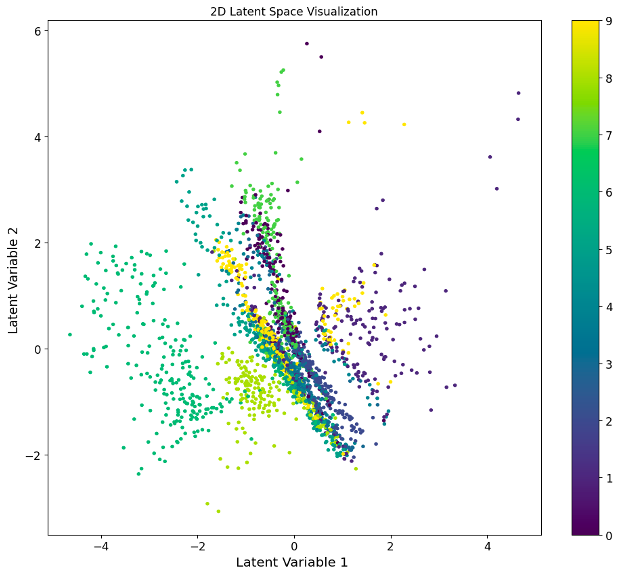
\includegraphics[width=\linewidth]{mlp_vae_lat.png}
%         \caption{Latent Space Visualization on test data for VAE-MLP Model Trained for 50 epochs}
%         \label{fig:generated_audio}
%     \end{minipage}
% \end{figure}

% Since the model showed promise, we decided to observe the learned latent space representation of the model. However, the visualization clearly showed severe overlapping of the learned representations for certain digits (especially for digits 0,1,2,3, and 9), indicating the model has not learned distinctive representations for each of the digits yet. Observing the loss plot again, it was evident that while the model was learning, there remained room for additional improvement since both the losses displayed potential for further decrease (that is the losses were not observed to be saturated) in loss and learning the representations better. We therefore decided to train the model for more epochs.

% \subsubsection{VAE-MLP (100 Epochs)}
% The loss plot for the VAE-MLP model trained for 100 epochs showed limited improvement and instead displayed instability in the model. After approximately 70 epochs, both the training and validation losses exhibited no proper decrement. This discrepancy made it challenging to conclusively determine if the model suffered from underfitting or overfitting due to its unstable behavior.

% \begin{figure}[htbp]
%     \centering
%     \begin{minipage}[b]{0.45\linewidth}
%         \centering
%         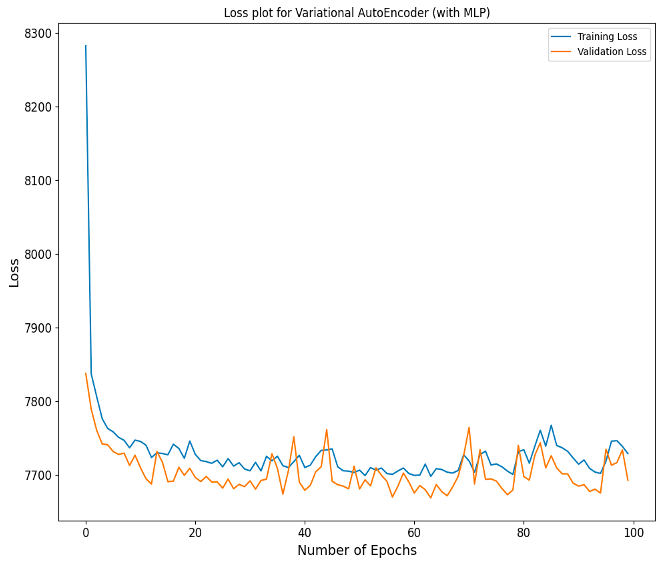
\includegraphics[width=\linewidth]{100.png}
%         \caption{Loss Curves for VAE-MLP Model trained for 100 epochs}
%         \label{fig:gen_stft}
%     \end{minipage}
%     \hfill
%     \begin{minipage}[b]{0.45\linewidth}
%         \centering
%         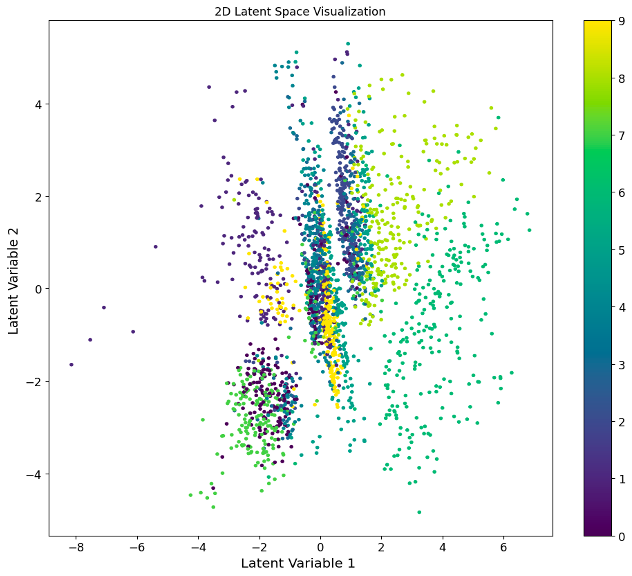
\includegraphics[width=\linewidth]{lat_100.png}
%         \caption{Latent Space Visualization on test data for VAE-MLP Model Trained for 100 epochs}
%         \label{fig:generated_audio}
%     \end{minipage}
% \end{figure}


% Despite its instability, a latent space visualization showcased improved representations compared to the earlier model. We can clearly observe in the figure above that the previously overlapping representations for digits 1 and 9 are now more distinct in comparison. The representations for other digits were observed to be distinct too in comparison however, the model seemed to fail to learn proper representation for 1 and 7, performing worse than the previous model.

% \subsubsection{Regularized VAE-MLP (100 Epochs)}
% Despite the ambiguous insights drawn from the previous model's loss plot, we adopted an intuitive approach, presuming that extended training epochs could enhance the model's performance rather than diminish it unless it was overfitting. Consequently, we opted to regularize the model and maintain the same number of training epochs. A dropout regularization rate of 30\% was implemented after each dense layer within both the encoder and decoder architectures.

% \begin{figure}[htbp]
%     \centering
%     \begin{minipage}[b]{0.45\linewidth}
%         \centering
%         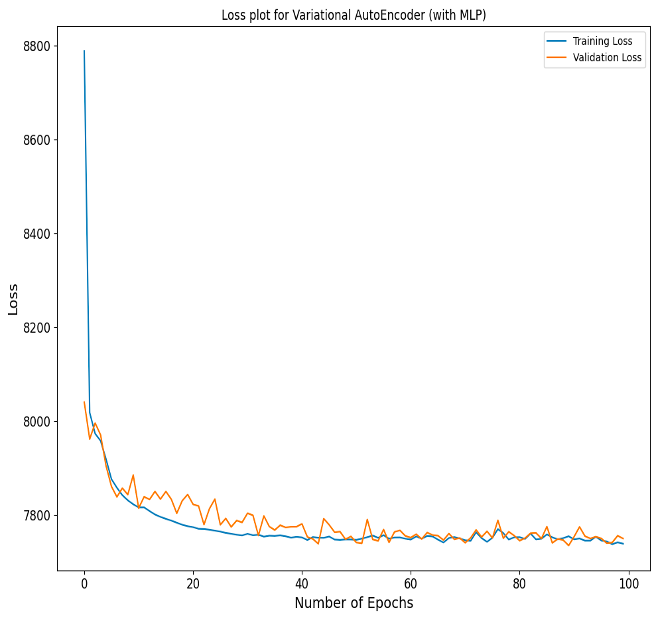
\includegraphics[width=\linewidth]{100r.png}
%         \caption{Loss Curves for regularized VAE-MLP Model trained for 100 epochs}
%         \label{fig:gen_stft}
%     \end{minipage}
%     \hfill
%     \begin{minipage}[b]{0.45\linewidth}
%         \centering
%         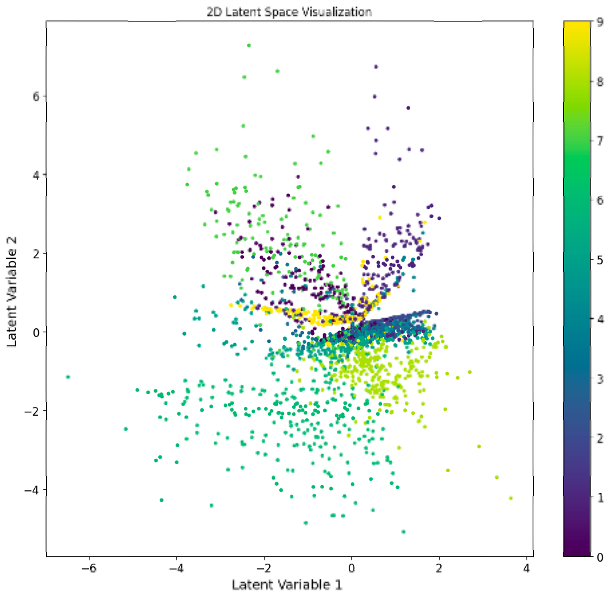
\includegraphics[width=\linewidth]{latr.png}
%         \caption{Latent Space Visualization on test data for regularized VAE-MLP Model Trained for 100 epochs}
%         \label{fig:generated_audio}
%     \end{minipage}
% \end{figure}


% Upon observing the subsequent loss plot and latent space visualization, notable findings surfaced. The model demonstrated increased stability, as indicated by both losses exhibiting a consistent downward trend, persisting until the final epoch. This indicated continual loss reduction throughout the training process. Examination of the latent space revealed more distinct and refined representations for each digit in comparison to both preceding models. Certain digits, namely 0, 5, 6, 7, 8, and 9, displayed sparser representations with reduced sample overlap. However, challenges persisted as the model encountered difficulty in learning distinct representations for digits 1, 2, 3, and 4.

% \subsection{VAE with CNN Models}

% \subsubsection{VAE-CNN (50 Epochs)}
% After employing MLP as encoding and decoding layers for VAE, we explored the use of CNN layer to do the encoding and decoding task. The architecture defined in section 3.3.2 was used to train the extracted STFT features.

% Initially, the model was trained for 50 epochs, and subsequently, the loss curves and latent space were scrutinized. The plotted loss curves indicated a consistent decrease in both training and validation losses until approximately 16 epochs. Beyond this point, the training loss continued to decrease, while the validation loss plateaued, signifying a case of overfitting. This variation, with the validation loss persisting higher than the training loss, explained that the model excelled on the training data (hence the low training loss) but struggled when generalizing to unseen data (resulting in the higher validation loss).

% \begin{figure}[htbp]
%     \centering
%     \begin{minipage}[b]{0.45\linewidth}
%         \centering
%         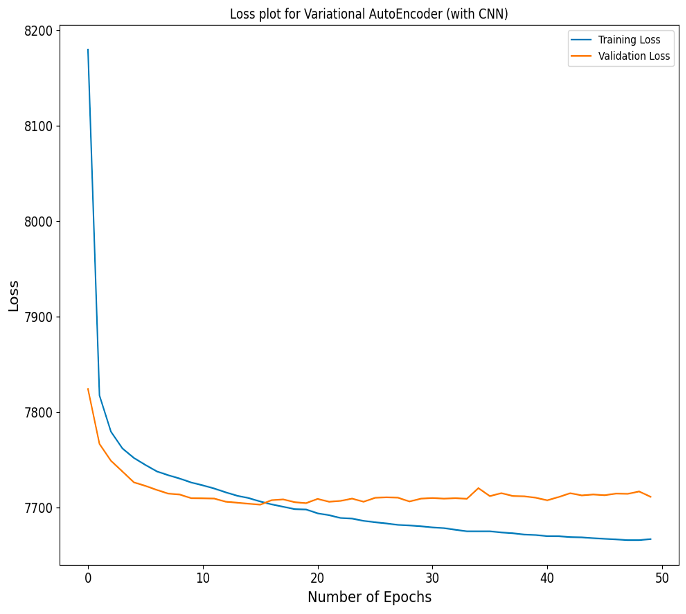
\includegraphics[width=\linewidth]{50c.png}
%         \caption{Loss Curves for VAE-CNN Model trained for 50 epochs}
%         \label{fig:gen_stft}
%     \end{minipage}
%     \hfill
%     \begin{minipage}[b]{0.45\linewidth}
%         \centering
%         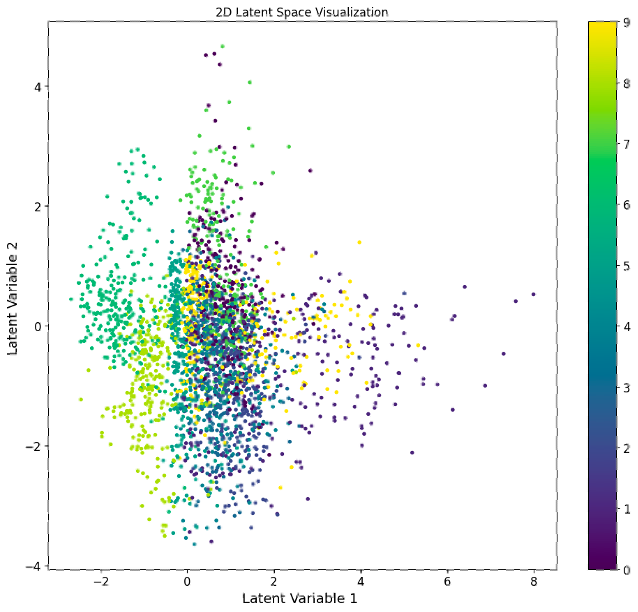
\includegraphics[width=\linewidth]{50clat.png}
%         \caption{Latent Space Visualization on test data for VAE-CNN Model Trained for 50 epochs}
%         \label{fig:generated_audio}
%     \end{minipage}
% \end{figure}


% Examining the latent space visualization provided further insights into the model's performance. The representations learned by the model appeared highly overlapped, implying an inability to distinguish unique representations for each digit. Only digits 6 and 8 exhibited somewhat distinctive representations amidst the overall lack of separation. Consequently, this model emerged as the worst-performing model among those tested.

% \subsubsection{Regularized VAE-CNN (50 Epochs)}
% As the prior VAE-CNN model exhibited clear signs of overfitting, we sought to address this issue by incorporating regularization techniques. We regularized the model using L2 regularizers (with regularization parameter (\(\lambda\)= 0.001) for the filters of the convolutional layer and 20\% dropout for the dense layers. The model was then trained on the same number of epochs (50) and the performance was observed using the loss and latent space plots.

% The loss plots showed a consistent and monotonic decline in both training and validation losses, indicating a resolution of the overfitting problem witnessed in the previous model. Notably, the decreasing loss values persisted throughout the entire training duration, suggesting continuous learning up to the final epoch.

% \begin{figure}[htbp]
%     \centering
%     \begin{minipage}[b]{0.45\linewidth}
%         \centering
%         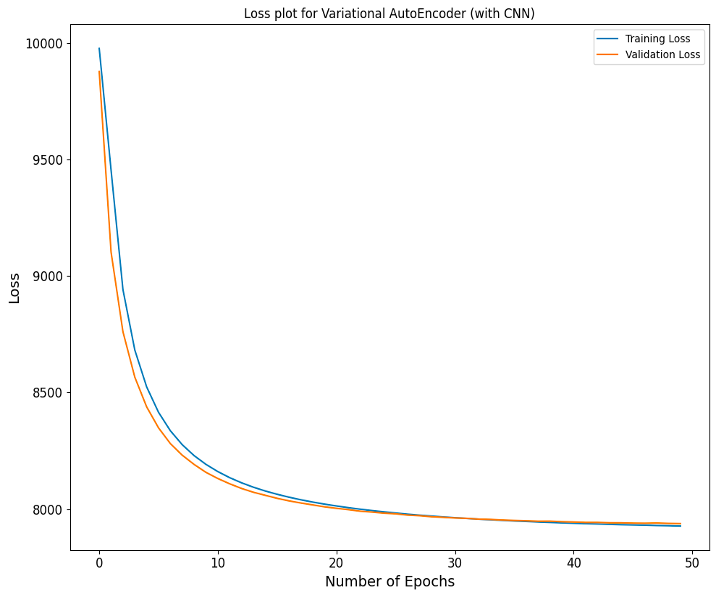
\includegraphics[width=\linewidth]{100cr.png}
%         \caption{Loss Curves for regularized VAE-CNN Model trained for 50 epochs}
%         \label{fig:gen_stft}
%     \end{minipage}
%     \hfill
%     \begin{minipage}[b]{0.45\linewidth}
%         \centering
%         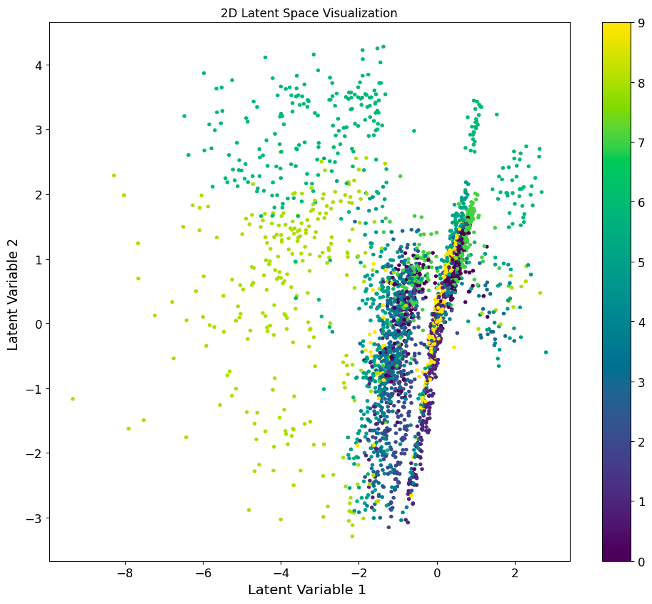
\includegraphics[width=\linewidth]{latcr.png}
%         \caption{Latent Space Visualization on test data for regularized VAE-CNN Model Trained for 50 epochs}
%         \label{fig:generated_audio}
%     \end{minipage}
% \end{figure}

% Analysis of the learned latent space exhibited enhanced performance compared to the previous VAE-CNN model, as the representations appeared more distinct. However, challenges persisted as the model struggled to effectively learn representations for all digits, demonstrating commendable performance solely for digits 4, 5, 6, 7, and 8. Despite exhibiting favorable loss curves, the model's overall improvement was marginal, ultimately underperforming compared to all VAE-MLP models evaluated.

% \begin{table}
% \centering
% \caption{Summary of the Model Outputs}
% \label{tab:my_table}
% \begin{tabular}{ l  l  l  l  l  l }

% Metrics / Models& \textbf{MLP-VAE 
% Model 1}& \textbf{MLP-VAE 
% Model 2}& \textbf{MLP-VAE 
% Regularized Model}& \textbf{CNN-VAE 
% Model 1}& \textbf{CNN-VAE 
% Regularized 
% Model}\\

% \textbf{Epochs} & 50 & 100 & 100 & 50 & 50 \\

% \textbf{Training Time
% (on Quadro k2200)}& 2.1 hrs& 5.3 hrs& 6.1 hrs& 18.7 hrs& 20.41 hrs\\

% \textbf{Training Loss} & 7673.74 & 7728.95 & 7738.79 & 7927.34 & 7987.90 \\

% \textbf{Validation Loss} & 7667.33 & 7697.56 & 7749.78 & 7937.97 & 7989.33 \\

% \textbf{Test Loss} & 7692.69 & 7707.67 & 7773.57 & 7962.82 & 7993.68 \\


% \end{tabular}

% \end{table}

